\documentclass[a4paper]{article}
\usepackage{hr-paper}

\title{Chinese Character Recognition}

\author{J.F. van Wezel}

\affil{University of Groningen}
\date{\today}

\newcommand{\numberofruns}{$500$ }
\newcommand{\N}{$N = 20$ }
\newcommand{\PS}{$P = 0.70, 0.75,\dots,3}
\begin{document}
\maketitle

%!TEX root = ../hr-paper.tex
\section{Introduction} % (fold)
\label{sec:introduction}



Introduction to the field

Why prepossessing is important

	- Noise reduction
	- Finding characters

Other methods and research done in this field.

Something about how a  (my version) is most of the times is a better solution than an extreme form.

The entire introduction should logically end at the research question and thesis statement or hypothesis.

	research question 	- How does the implemented segmentation method perform (in comparison with existing methods?)
	hypothesis			- Its probably oke for the time commited and the amount of work put in to it.


% section introduction (end)

%!TEX root = ../hr-paper.tex
\section{Dataset} % (fold)
\label{sec:dataset}

This section will shed light on the used dataset. It will show some examples of the noise encountered and problems that needed to be solved to achieve the segmented images.

- size of the dataset
- amount of labels
- amount of unique labels
- amount of unique charecters in the chinese language
- amount of fonts
- a little bit more about the individual fonts

- different kinds of noise in the dataset
	-Rotation
	-Lines
	-Round shapes
	-Multi line chars
	-weird chars
%!TEX root = ../hr-paper.tex
\section{Method} % (fold)
\label{sec:method}

The 

\subsection{Segmentation}


The Chinese characters were supplied in greyscale strokes of characters in the western orientation (from left to right).

%Otsu, N., "A Threshold Selection Method from Gray-Level Histograms," IEEE Transactions on Systems, Man, and Cybernetics, Vol. 9, No. 1, 1979, pp. 62-66.
In order to segment the characters from an image a combination of methods is used. First the image is binarized. Binarization is done by applying a Gaussian filter on the image to remove some of the noise. Then Otsu's method of finding a threshold is used. The image is then binarized using this threshold.

\todo[inline]{TODO: Add references for Otsu and gausian filtering}

After binarization the image is rotated. This is done because most images in the dataset are titled slightly. This is probably due to some variations in the orientation of the paper during the scanning process. Rotation is done by resizing the image in the vertical direction to half its size. The idea behind this is that the characters will be squeezed together and form a horizontal line this line can then be used to find the optimal rotation. this is done by taking the horizontal densities. The maximum densities are saved for the different rotations (between $+1\degree$ and $-1\degree$). The rotation with the largest maximum density is where the line is likely to be the most horizontal. This is taken as the optimal rotation. 


After the characters are rotated the vertical location of the characters are located by taking the horizontal densities. The densities are smoothed by using a averaging filter with ten of the neighboring densities. Then the densities are thresholded. The threshold is determined by taking $0.1 \times imageWidth$. From the resulting vertical areas the largest area is taken. This is based on the assumption that characters will produce the most wide peak in horizontal densities. For example many of the images hold a horizontal line above or beneath the characters. This line will produce a narrow but high peak when the horizontal densities are taken. The characters will in this case produce a lower and wider peak. After the determination of the vertical location of the characters the rest of the image is removed leaving only a horizontal stroke of characters.

\todo[inline]{TODO: Add image of the densities}


We are left with a isolated stroke of characters. In order to find the characters in this stroke the connected components are taken. This will give us a list of all the connected components in the image. If multiple components are above each other we assume that these components are part of the same character. These components are merged. Some components are not directly on top of each-other. It is determent how much the components overlap vertically. If the overlapping width is $0.4$ times the width of the width of the smaller of the two components, they are merged. 

After merging vertically we are left with a list of components that might be outliers in terms of width in comparison with the mean width of the characters in the supplied labeled dataset. In order to recognize outliers the mean and standard deviation was calculated from the characters in the labeled dataset. A component is deemed a small out-lier if:

\begin{equation}
C_w < \mu_w + 2 \sigma_w 
\end{equation}

and big if:

\begin{equation}
C_w > \mu_w + 2 \sigma_w 
\end{equation}

Here $C_w$ is the component's width, $\mu_w$ is the mean width ,and $\sigma_w$ is the standard deviation in width.


Small components that are characters on their own are often preceded and followed by more white space than components that form a character with the component left or right from it. The small characters are inspected on this feature and it is determined if this small component is actually a character. Some small components are just noise. If a component is too small, has too much black pixels or too much white pixels, it is recognized as noise and it is removed from the list of components. 

\todo[inline]{TODO: At the moment these determinations are made by chosen thresholds. But these thresholds can be extracted from the labeled dataset}

All that is left in the list of small components are expected to be components of characters. The components are merged with their left or right neighbor based on the width the newly merged component will have. Small components merge with the component (left or right) that together will have the smallest width. If however both neighboring components are deemed as big by the outliers detection, no merging will take place. The component is measured after merging. If the merged components is still small, the algorithm will try to merge it again with its left or right neighbor.

\todo[inline]{TODO: Sometimes 2 characters are seen as one because of some noise above the characters or because they are both small. This can be detected by taking the components that are deemed big and see if they can be separated in two or more components if there is a lot of white space in between them or by looking at the vertical densities.}


\subsection{Feature Extraction}

\subsection{Classification}

% section method (end

%!TEX root = ../hr-paper.tex
\section{Experiment} % (fold)
\label{sec:experiment}

This section will show by example how the segmented dataset is validated.  

% how the labels are used with our images to validate our images.
% IOU


\begin{figure}[ht]
  \centering
  \begin{subfigure}{0.25\textwidth}
    \centering
    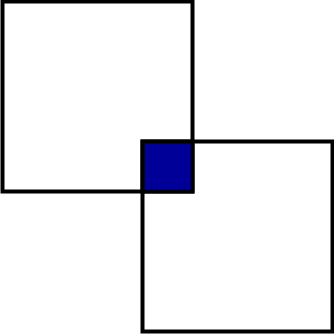
\includegraphics[width=\textwidth]{./images/experiment/intersection.png}
    \caption{Intersected area}
    \label{fig:experiment:intersection}
  \end{subfigure}
  \begin{subfigure}{0.25\textwidth}
    \centering
    
\includegraphics[width=\textwidth]{./images/experiment/union.png}
    \caption{Area of the union}
    \label{fig:experiment:union}
  \end{subfigure}
  \caption{Method of validating the segmented data (intersection over union)}
  \label{fig:experiment:iou}
\end{figure}

In order to validate the segmented images obtained by the segmentation the intersection over union is used. As shown in figure \ref{fig:experiment:intersection} the intersection between two boxes is the area that overlaps between these boxes. The union over two boxes give the area both the boxes occupy (figure \ref{fig:experiment:union}). The fraction between the intersection and the union tells us how well the boxes fit on top of each other. With this fraction the performance of the segmentation can be measured.

Because the characters consist mainly of black pixels, and the location of the box is arbitrary, the intersection over union is done only over the black pixels in both boxes. This is done by binerizing the original image and taking its complement. The complement is taken so black pixels will be represented by ones and white pixels by zeros. Now the labeled box and a segmented box are both printed on a white background the size of the original image. This results in two binary images on which an And is the same as the intersection, an Or is the same as a union. Summing the result from these operations give us the needed scalers to perform the intersection over union fraction.

 \begin{figure}[ht]
  \centering
  \begin{subfigure}{0.24\textwidth}
    \centering
    
\includegraphics[width=0.7\textwidth]{./images/experiment/label.png}
    \caption{Label image}
    \label{fig:experiment:label}
  \end{subfigure}
  \begin{subfigure}{0.24\textwidth}
    \centering
    
\includegraphics[width=0.7\textwidth]{./images/experiment/found.png}
    \caption{Segmented image}
    \label{fig:experiment:found}
  \end{subfigure}
    \begin{subfigure}{0.24\textwidth}
    \centering
    
\includegraphics[width=0.7\textwidth]{./images/experiment/and.png}
    \caption{Label and Segmented}
    \label{fig:experiment:and}
  \end{subfigure}
  \begin{subfigure}{0.24\textwidth}
    \centering
    
\includegraphics[width=0.7\textwidth]{./images/experiment/or.png}
    \caption{Label or Segmented}
    \label{fig:experiment:or}
  \end{subfigure}
  \caption{Example of intersection over union on a segmented character in the dataset, $IoU \approx 0.73$. The character used is the twelfth character in the image shown in figure \ref{fig:dataset:chinese:example}. }
  \label{fig:experiment:iou:example}
\end{figure}

In order to be able to say anything about the performance of the segmentation results will be thresholded from an intersection over union rate from 0.1 to 10. if the intersection over union is lower than 0.1 the boxes are not touching each other enough.


% section experiment (end)

%!TEX root = ../hr-paper.tex
\newpage
\section{Results} % (fold)
\label{sec:results}

This section will show the direct results of the intersection over union from the segmentation system. It will also show some cases where the segmentation seemed to have failed and where it succeeded.


\begin{minipage}{\linewidth}
\flushleft
\captionof{table}{IoU Results} \label{tab:results:iou} 
\begin{tabular}{ c c c c c c c c c c}
\hline
\hline
0.1		&	0.2		&	0.3		&	0.4		&	0.5		&	0.6		&	0.7		&	0.8		&	0.9		&	1		\\
0.988	&	0.973	&	0.948	&	0.905	&	0.841	&	0.769	&	0.704	&	0.631	&	0.532	&	0.117	\\
\hline
\end{tabular}\par
\bigskip
The results from the segmented characters with the labeled data from the dataset.
\end{minipage}


\begin{minipage}{\linewidth}
\flushleft
\captionof{table}{Knn base-set, Sobel} \label{tab:results:base:sobel} 
\begin{tabular}{r|ccccc}
\textbf{K} & \textbf{Cityblock} & \textbf{Euclidean} & \textbf{Euclidean(norm)} & \textbf{Mahalanobis} & \textbf{Cosine} \\
\hline
\hline
1  & 0.6887    & 0.6689    & 0.7219          & 0.7294      & 0.7234 \\
2  & 0.5900    & 0.5660    & 0.6308          & 0.6517      & 0.6289 \\
3  & 0.5517    & 0.5249    & 0.5984          & 0.6173      & 0.5964 \\
4  & 0.5217    & 0.4953    & 0.5698          & 0.5926      & 0.5674 \\
5  & 0.5018    & 0.4736    & 0.5551          & 0.5822      & 0.5528 \\
6  & 0.4958    & 0.4635    & 0.5450          & 0.5754      & 0.5439 \\
7  & 0.4943    & 0.4598    & 0.5445          & 0.5761      & 0.5420 \\
8  & 0.4927    & 0.4567    & 0.5440          & 0.5734      & 0.5405 \\
9  & 0.4933    & 0.4552    & 0.5420          & 0.5730      & 0.5408 \\
10 & 0.4914    & 0.4525    & 0.5387          & 0.5726      & 0.5405 \\
11 & 0.4871    & 0.4514    & 0.5365          & 0.5701      & 0.5416 \\
12 & 0.4857    & 0.4486    & 0.5367          & 0.5680      & 0.5381 \\
13 & 0.4856    & 0.4486    & 0.5354          & 0.5674      & 0.5377 \\
14 & 0.4829    & 0.4473    & 0.5334          & 0.5658      & 0.5361 \\
15 & 0.4824    & 0.4455    & 0.5311          & 0.5639      & 0.5335 \\
16 & 0.4835    & 0.4433    & 0.5295          & 0.5618      & 0.5335 \\
17 & 0.4823    & 0.4421    & 0.5294          & 0.5608      & 0.5326 \\
18 & 0.4815    & 0.4412    & 0.5269          & 0.5586      & 0.5321 \\
19 & 0.4811    & 0.4407    & 0.5237          & 0.5568      & 0.5314 \\
20 & 0.4794    & 0.4400    & 0.5219          & 0.5563      & 0.5308
\end{tabular}\par
\bigskip
The classification rates of the feature extracted characters from the labeled base-set. Feature extraction was done with the Sobel filter and  Knn with $K$ from 1 to 20. 
\end{minipage}

\begin{minipage}{\linewidth}
\flushleft
\captionof{table}{Knn base-set, Prewit} \label{tab:results:base:prewit} 
\begin{tabular}{r|ccccc}
\textbf{K} & \textbf{Cityblock} & \textbf{Euclidean} & \textbf{Euclidean(norm)} & \textbf{Mahalanobis} & \textbf{Cosine} \\
\hline
\hline
1          & 0.6509             & 0.7172             & 0.7219                   & \textbf{0.7432}       & 0.6241          \\
2          & 0.5410             & 0.6242             & 0.6308                   & 0.6647               & 0.5057          \\
3          & 0.4996             & 0.5964             & 0.5984                   & 0.6349               & 0.4616          \\
4          & 0.4649             & 0.5685             & 0.5698                   & 0.6146               & 0.4190          \\
5          & 0.4458             & 0.5534             & 0.5551                   & 0.6037               & 0.3906          \\
6          & 0.4362             & 0.5470             & 0.5450                   & 0.5978               & 0.3748          \\
7          & 0.4297             & 0.5447             & 0.5445                   & 0.5955               & 0.3698          \\
8          & 0.4265             & 0.5425             & 0.5440                   & 0.5904               & 0.3674          \\
9          & 0.4264             & 0.5413             & 0.5420                   & 0.5896               & 0.3656          \\
10         & 0.4260             & 0.5389             & 0.5387                   & 0.5902               & 0.3646          \\
11         & 0.4255             & 0.5375             & 0.5365                   & 0.5886               & 0.3600          \\
12         & 0.4247             & 0.5373             & 0.5367                   & 0.5852               & 0.3599          \\
13         & 0.4252             & 0.5372             & 0.5354                   & 0.5812               & 0.3593          \\
14         & 0.4257             & 0.5348             & 0.5334                   & 0.5816               & 0.3598          \\
15         & 0.4259             & 0.5326             & 0.5311                   & 0.5807               & 0.3587          \\
16         & 0.4257             & 0.5293             & 0.5295                   & 0.5797               & 0.3594          \\
17         & 0.4253             & 0.5262             & 0.5294                   & 0.5771               & 0.3583          \\
18         & 0.4282             & 0.5252             & 0.5269                   & 0.5761               & 0.3580          \\
19         & 0.4274             & 0.5235             & 0.5237                   & 0.5741               & 0.3561          \\
20         & 0.4272             & 0.5219             & 0.5219                   & 0.5719               & 0.3561 
\end{tabular}\par
\bigskip
The classification rates of the feature extracted characters from the labeled base-set. Feature extraction was done with the Prewit filter and  Knn with $K$ from 1 to 20. 
\end{minipage}



\begin{minipage}{\linewidth}
\flushleft
\captionof{table}{Knn segmented-set, Sobel} \label{tab:results:seg:sobel} 
\begin{tabular}{r|ccccc}
\textbf{K} & \textbf{Cityblock} & \textbf{Euclidean} & \textbf{Euclidean(norm)} & \textbf{Mahalanobis} & \textbf{Cosine} \\
\hline
\hline
1  & 0.8054    & 0.8305    & 0.8275          & 0.8179      & 0.7940 \\
2  & 0.6865    & 0.7267    & 0.7252          & 0.7149      & 0.6676 \\
3  & 0.6274    & 0.6789    & 0.6720          & 0.6621      & 0.6091 \\
4  & 0.5911    & 0.6438    & 0.6384          & 0.6322      & 0.5732 \\
5  & 0.5748    & 0.6348    & 0.6308          & 0.6159      & 0.5557 \\
6  & 0.5672    & 0.6278    & 0.6271          & 0.6106      & 0.5503 \\
7  & 0.5693    & 0.6295    & 0.6267          & 0.6093      & 0.5456 \\
8  & 0.5666    & 0.6312    & 0.6269          & 0.6067      & 0.5449 \\
9  & 0.5665    & 0.6313    & 0.6245          & 0.6056      & 0.5438 \\
10 & 0.5671    & 0.6309    & 0.6235          & 0.6018      & 0.5429 \\
11 & 0.5644    & 0.6275    & 0.6204          & 0.5991      & 0.5441 \\
12 & 0.5601    & 0.6224    & 0.6193          & 0.5964      & 0.5403 \\
13 & 0.5601    & 0.6199    & 0.6145          & 0.5960      & 0.5390 \\
14 & 0.5594    & 0.6165    & 0.6127          & 0.5960      & 0.5374 \\
15 & 0.5593    & 0.6164    & 0.6090          & 0.5929      & 0.5390 \\
16 & 0.5580    & 0.6118    & 0.6061          & 0.5929      & 0.5363 \\
17 & 0.5579    & 0.6086    & 0.6034          & 0.5908      & 0.5358 \\
18 & 0.5557    & 0.6059    & 0.6012          & 0.5897      & 0.5351 \\
19 & 0.5545    & 0.6053    & 0.5978          & 0.5880      & 0.5344 \\
20 & 0.5552    & 0.6043    & 0.5977          & 0.5861      & 0.5312
\end{tabular}\par
\bigskip
The classification rates with the segmented and feature extracted characters. Feature extraction was done with the Sobel filter and  Knn with $K$ from 1 to 20. 
\end{minipage}


%knn prewit seg

\begin{minipage}{\linewidth}
\flushleft
\captionof{table}{Knn segmented-set, Prewit} \label{tab:results:seg:prewit} 
\begin{tabular}{r|ccccc}
\textbf{K} & \textbf{Cityblock} & \textbf{Euclidean} & \textbf{Euclidean(norm)} & \textbf{Mahalanobis} & \textbf{Cosine} \\
\hline
\hline
1          & 0.7701             & 0.7429             & 0.8229                   & \textbf{0.8254}      & 0.7456          \\
2          & 0.6281             & 0.5903             & 0.7129                   & 0.7234               & 0.5925          \\
3          & 0.5659             & 0.5149             & 0.6626                   & 0.6714               & 0.5223          \\
4          & 0.5209             & 0.4623             & 0.6303                   & 0.6442               & 0.4702          \\
5          & 0.4996             & 0.4319             & 0.6178                   & 0.6343               & 0.4396          \\
6          & 0.4893             & 0.4223             & 0.6076                   & 0.6281               & 0.4257          \\
7          & 0.4877             & 0.4167             & 0.6107                   & 0.6281               & 0.4222          \\
8          & 0.4857             & 0.4106             & 0.6089                   & 0.6249               & 0.4146          \\
9          & 0.4846             & 0.4066             & 0.6060                   & 0.6234               & 0.4126          \\
10         & 0.4823             & 0.4062             & 0.6009                   & 0.6204               & 0.4137          \\
11         & 0.4848             & 0.4028             & 0.5993                   & 0.6202               & 0.4140          \\
12         & 0.4846             & 0.4022             & 0.5974                   & 0.6178               & 0.4121          \\
13         & 0.4839             & 0.4023             & 0.5961                   & 0.6162               & 0.4107          \\
14         & 0.4826             & 0.4002             & 0.5941                   & 0.6128               & 0.4100          \\
15         & 0.4815             & 0.3991             & 0.5923                   & 0.6121               & 0.4077          \\
16         & 0.4819             & 0.3964             & 0.5906                   & 0.6096               & 0.4076          \\
17         & 0.4789             & 0.3947             & 0.5875                   & 0.6100               & 0.4067          \\
18         & 0.4792             & 0.3943             & 0.5855                   & 0.6078               & 0.4068          \\
19         & 0.4799             & 0.3935             & 0.5829                   & 0.6067               & 0.4067          \\
20         & 0.4800             & 0.3916             & 0.5810                   & 0.6047               & 0.4069         
\end{tabular}\par
\bigskip
The classification rates with the segmented and feature extracted characters. Feature extraction was done with the Prewit filter and  Knn with $K$ from 1 to 20. 
\end{minipage}

%2comps





% - image to big due to line noise
% image to big due to other noise
% correct small
% 2 in one
% - 1.5

% section results (end)

%!TEX root = ../hr-paper.tex
\section{Discussion} % (fold)
\label{sec:discussion}

% section discussion (end)

%!TEX root = ../hr-paper.tex
\section{Conclusion} % (fold)
\label{sec:conclusion}

Based on the example shown in the results section and discussed in the discussion section we must conclude that the segmentation achieved seems good but could be better when more work is put in to it. Most examples handled in the discussion concluded in the same thing. Namely that some part of the system was faulty or that some parameter still needed to be tweaked more. Almost all problems shown could be handled by the methods implemented in the system. The connected components implementation together with horizontal and vertical projection shows promise and should (if worked out more) be  able to  achieve better results. This work however shows that a hybrid form can achieve segmentation with the best of both worlds.


% section conclusion (end)
\bibliographystyle{plain}
\bibliography{bibliography}

% \begin{figure}[hbt]
% 	\centering
% 		\includegraphics[width=0.5\textwidth]{./img/colormap/colormap.png}
% 		\caption{Colourmap which maps (initial) values of $P$ and $x$ to unique colours.}
% 		\label{fig:app:colormap}
% \end{figure}






\end{document}
